\section{方法}
\label{sec:method}

\subsection{预算、索引与实际送入模型的特征}
\label{sec:overview}

给定图像和问题，视觉塔产生 $N$ 个与原始 patch 对齐的位置。LLaVA-1.5 使用 CLIP-ViT-L/14-336，网格为 $24\times 24$，故 $N{=}576$，语言模型有 $L{=}32$ 层~\cite{llava15,clip}。记第 $\ell$ 个 Decoder block 实际处理的视觉 token 数为 $K_\ell$。视觉 token-layer 预算、层平均数量和相对完整视觉序列的比例分别是
\begin{equation}
 W=\sum_{\ell=1}^{L}K_\ell,\qquad
 \bar K=W/L,\qquad
 \rho_W=W/(LN).
 \label{eq:budget}
\end{equation}
$W$ 只累计各层看见的视觉 token 个数。它不包含文本长度，也不等于 FLOPs、延迟或显存。

选择发生在两个地方，如图~\ref{fig:framework}。语言模型之前，方法确定入口集合 $S$，且 $|S|{=}K_0$。语言模型内部，指定 block 结束后把当前存活集合嵌套地收成更小的集合。两条路径使用的特征不同。选择描述只参与比较位置；真正进入投影器和 Decoder 的，是视觉塔倒数第二个 block 的 patch 特征按索引取出的那些行。代码在选择前检查这些行与投影器输入逐元素一致。被删位置不再出现在后续 block 的隐藏状态里，其 RoPE 位置编号保持删除前的原始编号，不重新排成连续整数。

\begin{figure*}[t]
 \centering
 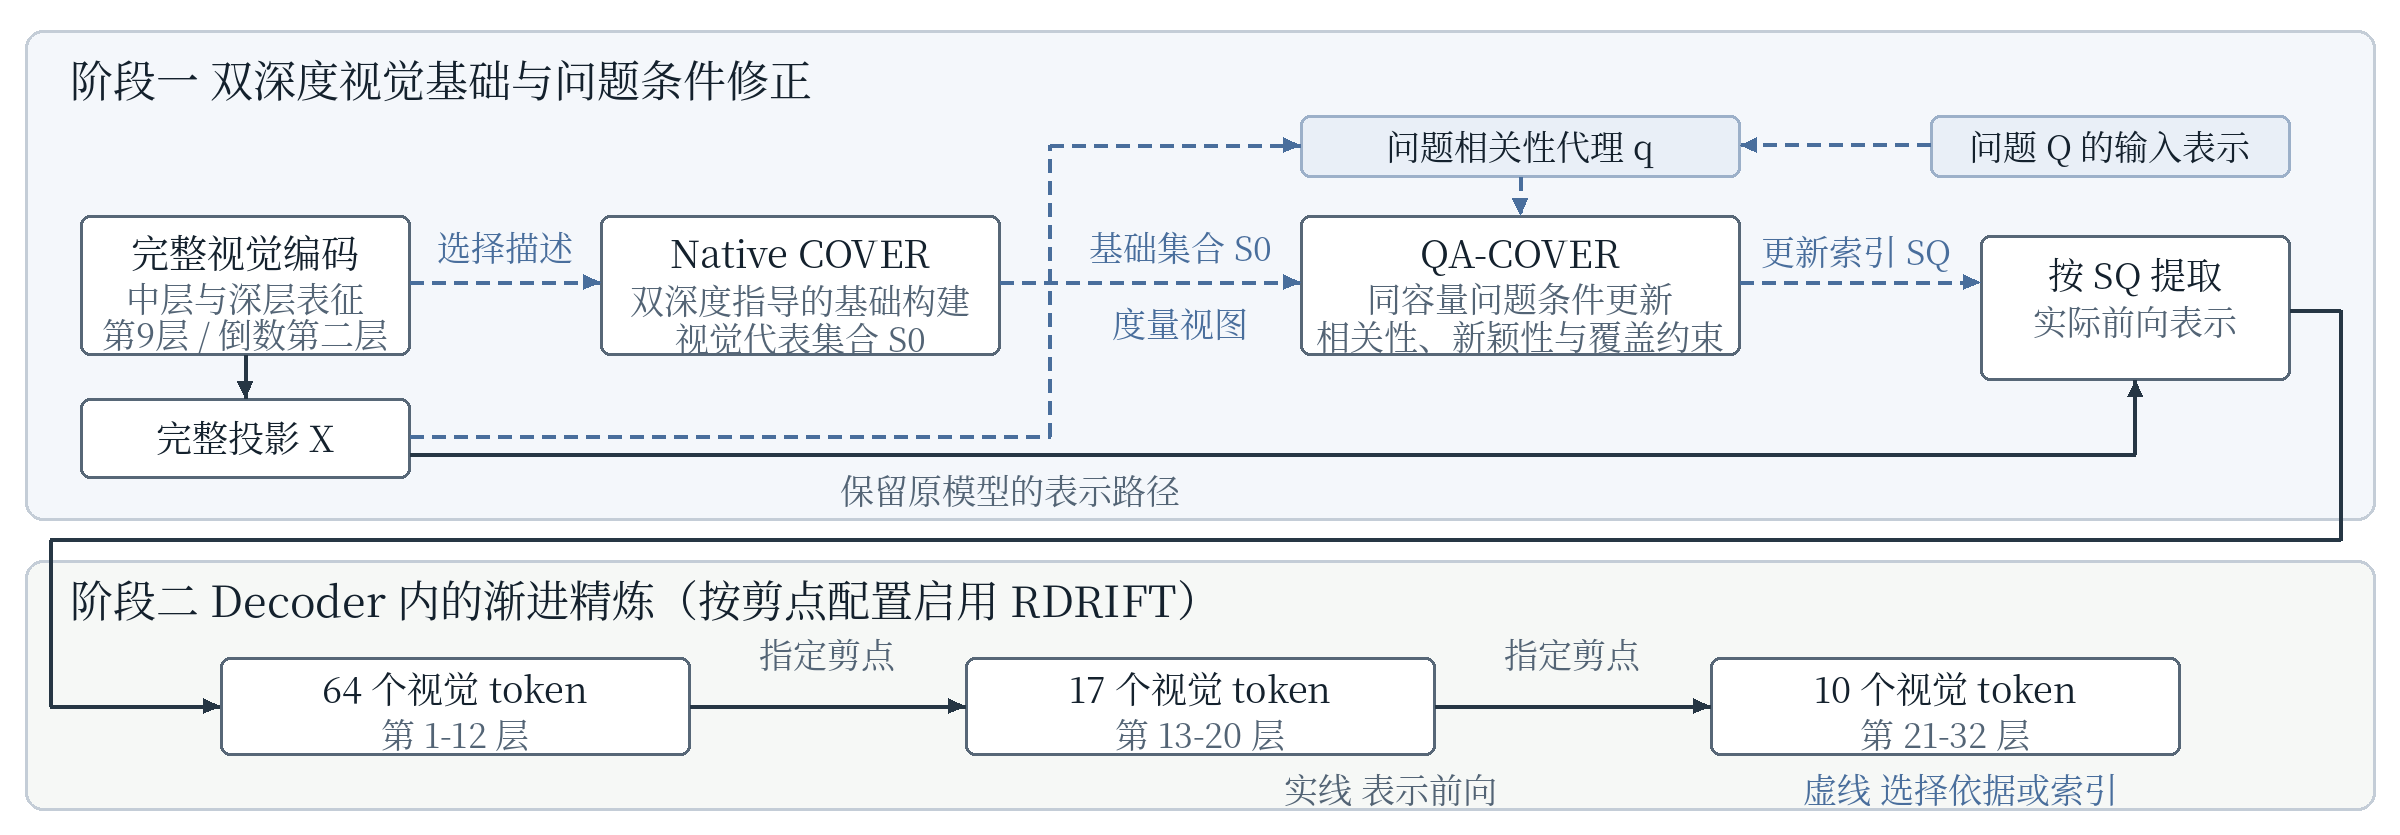
\includegraphics[width=\textwidth]{figures/bela_framework.png}
 \caption{BELA 的两条路径。虚线是选择描述或索引，实线是进入投影器与 Decoder 的原始特征。初始化用双深度显著性与 $4\times 4$ 空间原型补足锚点；问题条件更新在另一套全体位置覆盖上做有限次交换。图中层号从 1 计：第 1--12、13--20、21--32 层分别对应正文从 0 计的 block 0--11、12--19、20--31。图中的秩漂移只用于第一次剪枝；第二次剪枝使用问题注意力。$64\!\rightarrow\!17\!\rightarrow\!10$ 是 $W{=}1024$ 的数量日程。}
 \label{fig:framework}
\end{figure*}

\subsection{双深度描述与空间原型初始化}
\label{sec:visualbase}

记 CLIP 的 hidden state 包含嵌入输出。第 9 个 Transformer block 的 patch 输出记为 $F^{(9)}$，对应 \texttt{hidden\_states[9]}，其 CLS 到 patch 的注意力取 \texttt{attentions[8]}。倒数第二个 block 的 patch 输出记为 $F^{\mathrm{pen}}$，对应 \texttt{hidden\_states[-2]} 与 \texttt{attentions[-2]}。两层的第 $i$ 行都是同一个原始 patch。显著性是多头注意力中 CLS 对 patch 的和，不是先对头取平均再做 $\ell_1$：
\begin{equation}
 s^{(9)}_i=\sum_{h}A^{(9)}_{h,0,i},\qquad
 s^{\mathrm{pen}}_i=\sum_{h}A^{\mathrm{pen}}_{h,0,i}.
\end{equation}
报告配置取 $\beta{=}0.5$，融合分数与选择描述为
\begin{equation}
\begin{aligned}
 s_i&=(1-\beta)s^{\mathrm{pen}}_i+\beta s^{(9)}_i,\\
 z_i&=\big[\sqrt{1-\beta}\,\hat u(F^{\mathrm{pen}}_i);\;
           \sqrt{\beta}\,\hat u(F^{(9)}_i)\big].
\end{aligned}
\label{eq:dual}
\end{equation}
$\hat u$ 表示按通道做 $\ell_2$ 归一化，稳定项为 $10^{-12}$。$z_i$ 是两层宽度的拼接。对 CLIP-ViT-L，单层宽度为 1024，拼接后为 2048。这个描述用于选索引，不替换 $F^{\mathrm{pen}}$。

初始化调用既有的 REPLACE/COVER 规则，入口 $K_0{=}64$，替换名额 $b{=}32$。锚点是融合显著性最高的 $K_0-b{=}32$ 个位置。候选池不是锚点之外的全部位置，而是融合显著性前 $K_0$ 名之外的 $N-K_0$ 个位置；因此显著性排名第 33 到第 64 的位置既不是锚点，也不会被补入。把 $24\times 24$ 网格划成 $4\times 4$ 个格子，每格 $6\times 6$。令 $\hat z_i$ 为对 $z_i$ 再次归一化的结果，稳定项为 $10^{-8}$。格子 $g$ 的原型是落在该格中的锚点特征的均值，然后再归一化；空格子的原型为零向量。位置 $i$ 的效用是
\begin{equation}
 u_i=s_i\Big(1-\operatorname{clip}\big(\cos(\hat z_i,m_{g(i)}),0,1\big)\Big).
 \label{eq:native}
\end{equation}
空格子的原型是零向量，余弦为零，效用退化为显著性本身。初始集合 $S_0$ 由 32 个锚点和效用最高的 32 个池外位置组成，再按原始 patch 编号排序。这一步只执行一次，不迭代最大化下一节的覆盖函数 $C$。它与问题无关。

\subsection{问题条件的同容量交换}
\label{sec:queryupdate}

更新从 $S_0$ 出发，容量始终为 $K_0$。报告配置把显著性保护名额设为 0，因此交换阶段不再用 CLS 分数保护任何成员。问题代理与外部预计算分数二选一；本文的运行使用嵌入路径。先用已有的多模态投影器处理全部 $N$ 个 $F^{\mathrm{pen}}$ 行，得到与语言模型同宽的向量 $x_i$。问题 token 去掉模板词和标点，只保留内容片段；若内容片段为空，或原始分数的总体标准差低于 $0.008$，则保持 $S_0$ 不变。设内容片段的输入嵌入为 $\{e_t\}$，
\begin{equation}
\begin{gathered}
 \bar e=\frac{1}{|Q_c|}\sum_{t\in Q_c}e_t,\qquad
 a_i=\cos(x_i,\bar e),\\
 q_i=\sigma\Big(\operatorname{clip}\big(\frac{a_i-\operatorname{med}(a)}{2\,\operatorname{std}(a)},-8,8\big)\Big).
\end{gathered}
\label{eq:query}
\end{equation}
$\sigma$ 是 sigmoid，$\operatorname{clip}$ 把数值截到给定区间。标准差是总体标准差，分母的下限为 $10^{-12}$。偶数长度时中位数取排序后两个中间值中较低的一个。$q_i$ 是问题方向的代理，不是经过专门对齐训练的相关性概率。

覆盖使用式~\eqref{eq:dual} 的描述，并且只传入这一个视图。对每一行再次做 $\ell_2$ 归一化后，
\begin{equation}
\begin{aligned}
 G_{ij}&=\operatorname{clip}\big(\cos(z_i,z_j),0,1\big),\\
 C(S)&=\frac1N\sum_{i=1}^{N}\max_{j\in S}G_{ij},\\
 \nu(v\mid S)&=1-\max_{j\in S}G_{vj},\quad v\notin S.
\end{aligned}
\label{eq:coverage}
\end{equation}
$C(S)$ 是全体原始位置到当前集合的平均最近代表相似度。$\nu$ 只比较候选和当前集合，二者不是同一个量。$G$ 由截断余弦得到，不假设它是度量，也不把 $1-C(S)$ 解释成率失真。

每一轮都按当前集合重新排序候选，先前被移出的位置可以再次进入。集合外位置按 $q_v\nu(v\mid S)$ 取前 $P_a{=}16$ 个；集合内位置按
\begin{equation}
 p_{\mathrm{drop}}(u)=1-q_u+\frac12\max_{j\in S,\,j\neq u}G_{uj}
 \label{eq:drop}
\end{equation}
取前 $P_d{=}12$ 个。单元素集合的内部冗余取零。对一对 $(u,v)$，令 $S'=(S\setminus\{u\})\cup\{v\}$，$\Delta q=q_v-q_u$，$\Delta C=C(S')-C(S)$。可行条件为
\begin{equation}
 \Delta q\ge \gamma,\qquad
 \nu(v\mid S)\ge \tau_\nu,\qquad
 \Delta C\ge -\varepsilon,
 \label{eq:feasible}
\end{equation}
报告配置中 $\gamma{=}0.08$、$\tau_\nu{=}0.05$、$\varepsilon{=}0.005$。在可行对中最大化
\begin{equation}
 J(u,v)=\Delta q\,\nu(v\mid S)+\lambda\Delta C,
 \label{eq:swap}
\end{equation}
$\lambda{=}0.5$。实现取可行分数中的最大有限值，没有额外的 $J>0$ 判断。没有可行对，或已完成 $B{=}8$ 次交换时停止。$B$ 是上限，不保证每次样本都交换满 8 次。接受后按原始编号排序，得到 $S_Q$。

匹配随机对照保留同一次运行实际删除的位置和相同的净交换数，只把新增位置换成种子为 17 的随机位置。错配对照仍走式~\eqref{eq:query}--\eqref{eq:swap}，但问题向量来自固定的错配排列。

\subsection{移除损失与变化范围}
\label{sec:mechanism}

设 $R=S\setminus\{u\}$，空集的最大相似度为 0，并记 $b_i(R)=\max_{j\in R}G_{ij}$。一次交换的覆盖变化可以拆开：
\begin{equation}
\begin{aligned}
 D_C(u\mid S)&=C(S)-C(R)
  =\frac1N\sum_{i=1}^{N}[G_{iu}-b_i(R)]_+,\\
 A_C(v\mid R)&=\frac1N\sum_{i=1}^{N}[G_{iv}-b_i(R)]_+,\\
 \Delta C&=A_C(v\mid R)-D_C(u\mid S).
\end{aligned}
\label{eq:decomposition}
\end{equation}
$D_C$ 是 $u$ 对全体位置的不可替代程度，不等于 $1-q_u$。$A_C$ 是 $v$ 能把多少位置的最近代表提高，不等于 $\nu(v\mid S)$。式~\eqref{eq:feasible} 的覆盖门因此等价于加入补偿至少补上移除损失超出 $\varepsilon$ 的部分。

一个构造例子可以分开这两个量，它不是实验样本。100 个位置分成 50、49、1 的三簇，簇内相似度为 1，簇间为 0。保留前两簇各一个代表时 $C{=}0.99$。若用第三簇的唯一点替换第一簇的代表，该点相对当前集合的新颖性为 1，但覆盖降到 0.50：移除损失 0.50，加入补偿 0.01。高新颖性仍可能破坏大量已有代表关系。反过来，若答案恰好落在被拒绝的小簇里，平均覆盖约束也会留下它。所以 $C$ 保护的是特征代理下的代表关系，不是答案充分性。

设实际接受 $T\le B$ 次交换。一进一出和逐步门槛给出
\begin{equation}
\begin{gathered}
 |S_Q|=K_0,\qquad |S_Q\cap S_0|\ge K_0-T,\\
 C(S_Q)\ge C(S_0)-T\varepsilon,\\
 \sum_{i\in S_Q}q_i\ge \sum_{i\in S_0}q_i+T\gamma .
\end{gathered}
\label{eq:bounds}
\end{equation}
$K_0{=}64$、$T\le 8$ 时，最终集合至少还留着 56 个初始身份，累计覆盖下降不超过 $0.04$。这是式~\eqref{eq:coverage} 上的范围。可行对还满足 $J\ge \gamma\tau_\nu-\lambda\varepsilon=0.0015$，该下界来自门槛，不是实现里另写的判断。$J$ 依赖当前集合，算法没有在优化一个固定的全局目标，也没有次模近似保证。

\subsection{Decoder 内的两次精炼}
\label{sec:progressive}

$S_Q$ 对应的 $F^{\mathrm{pen}}$ 行与文本一起进入 Decoder。报告日程的段长是 12、8、12 层，保留数量是 64、17、10。实现在第 11 和 第 19 个 block（从 0 计数）结束后剪枝，事件写成 $11{:}17,19{:}10$。于是第 0--11 个 block 处理 64 个视觉 token，第 12--19 个处理 17 个，第 20--31 个处理 10 个：
\begin{equation}
 W=64\times 12+17\times 8+10\times 12=1024.
 \label{eq:schedule}
\end{equation}
因而 $\bar K{=}32$，$\rho_W{=}1/18\approx 5.56\%$，相对完整视觉序列少 $17/18\approx 94.44\%$。两次剪枝都从当前仍在序列中的视觉位置里选择，后一层的保留集合是前一层的子集。

两次使用的分数不同。第 0 个 block 之后，把问题到视觉的注意力行按问题 token 的原有顺序切成至多 4 段连续桶，保存每桶的平均。注意力本身先在完整合法前缀上做 softmax，再对头取平均，最后只留下视觉列。第一次剪枝时，用原始 patch 编号把这份浅层记录对齐到当前 64 个位置。令 $\bar\rho^{\mathrm{now}}$ 与 $\bar\rho^{\mathrm{old}}$ 分别为当前响应和浅层响应在桶上的平均。秩函数 $\pi$ 对向量做稳定的升序排序，最小值为 0、最大值为 1，并列项按原有顺序占据相邻秩，除以 $n-1$，不把并列项改成平均秩。第一次剪枝的分数是
\begin{equation}
 r_i=w\,\pi(\bar\rho^{\mathrm{now}})_i
 +(1-w)\big(\pi(\bar\rho^{\mathrm{now}})_i-\pi(\bar\rho^{\mathrm{old}})_i\big),
 \label{eq:rdrift}
\end{equation}
报告配置 $w{=}0.6$。保留 $r_i$ 最高的 17 个位置。这个排序直接决定第一次剪枝，不再使用该层的问题注意力 Top-$K$。第二次剪枝不读取式~\eqref{eq:rdrift}。它把问题位置上的视觉列注意力对问题 token 取平均，保留最高的 10 个。

隐藏状态在剪枝时按保留行聚集。报告运行的缓存策略是逐层局部缓存：已经执行过的 block 不回溯删除自己的 KV。因此前 12 层的缓存仍对应 64 个视觉位置，中间 8 层对应 17 个，最后 12 层对应 10 个。解码时，新 token 在浅层仍能读到入口集合的键值，在深层只能读到当时留下的视觉位置。末层存活数量不能代表全部缓存。一个入口位置后来被删掉，只说明它没有进入最后 12 层的隐藏状态，不能由此推出它的信息已经被文本状态吸收。

\subsection{执行过程与实际计算}
\label{sec:cost}

算法~\ref{alg:bela} 汇总上述顺序。视觉塔对全部 patch 做一次前向。问题代理额外调用一次全网格投影器，这 576 次投影不属于原生集合那一支的成本。式~\eqref{eq:coverage} 的相似度是 $N\times N$，描述宽度为两层通道数之和。每轮交换复用当前集合的最大和次大相似度，主要计算量随 $NK_0+NP_aP_d$ 增长。剪点上为了得到问题响应，实现会由该层的查询和键显式形成问题位置的 logits；报告运行的注意力后端是 SDPA，这几层的选择统计不能算成已被注意力内核完全吸收。

\begin{algorithm}[t]
\caption{BELA 的一次推理}
\label{alg:bela}
\begin{algorithmic}[1]
\REQUIRE 图像，问题，入口容量 $K_0$，段长与保留数
\STATE 视觉编码，取 $F^{(9)}$、$F^{\mathrm{pen}}$ 与 CLS 和显著性
\STATE 按式~\eqref{eq:dual}、\eqref{eq:native} 得到 $S_0$
\STATE $S\leftarrow S_0$；用全网格投影和内容嵌入算 $q$
\IF{$\operatorname{std}(q)\ge 0.008$}
 \STATE 由 $z$ 构造 $G$
 \FOR{$t=1,\ldots,\min(B,K_0,N-K_0)$}
  \STATE 按当前 $S$ 取加入池与移除池
  \IF{没有满足式~\eqref{eq:feasible} 的交换}
   \STATE \textbf{break}
  \ENDIF
  \STATE 按式~\eqref{eq:swap} 替换一对并重排 $S$
 \ENDFOR
\ENDIF
\STATE 以 $F^{\mathrm{pen}}_{S}$ 与文本进入 Decoder
\STATE block 11 后按式~\eqref{eq:rdrift} 留 17 个
\STATE block 19 后按问题注意力留 10 个
\STATE 聚集后续隐藏状态与位置编号
\STATE 已完成层的 KV 保持该层当时的长度
\ENSURE 各层视觉数量满足式~\eqref{eq:schedule}
\end{algorithmic}
\end{algorithm}

设第 $\ell$ 层序列长度为 $n_\ell=K_\ell+L_t$，$L_t$ 为文本长度，$d$ 与 $d_{\mathrm{ff}}$ 为隐藏宽度和前馈宽度。语言模型主体的计算规模是
\begin{equation}
 O\Big(\sum_{\ell=1}^{L}(n_\ell d^{2}+n_\ell^{2}d+n_\ell\,d\,d_{\mathrm{ff}})\Big).
 \label{eq:llmcost}
\end{equation}
式~\eqref{eq:budget} 只解释其中视觉 token 的个数。完整成本还要加上视觉塔、全网格投影、相似度、剪点上的问题--键乘积，以及解码时长短不一的缓存读取~\cite{flashattention,flashattention2,pagedattention}。
